\chapter{Used technologies}
\label{cap:usedtech}

\section{How to work with Gmail API}\label{sect:gmailapitech}
In order to be able to read and send emails, it is necessary to access to the user's email data. For this reason, the different ways to obtain this information were studied. One of them is the Gmail API, which allows developers to perform all the actions we need in an easy way.

Gmail API can be used in several programming languages such as Python, PHP, Go, Java, .NET, \ldots\phantom{ }Due to the greater number of examples in the starting guides of the Gmail API \citep{gmailAPI} and the previous knowledge that was already had of it, Python was chosen for the first contact with this technology.

The following tries to be a step-by-step explanation of what is necessary to know to access the user's Gmail account, create a message, send an email previously created, create and update a draft, reply a received message (for this it is necessary to know how to create an email) and read important information of message threads and individual emails (such as who is the sender, who has received the message, the subject, the date, the email's body, the attached files, \ldots). Methods of Gmail API resources (explained in Section \ref{ssect:gmailapi}) are studied to achieve this aim.

As we have seen in Section \ref{sssect:oauth}, in order to work with Gmail API, it is necessary to obtain the required OAuth 2.0 credentials. For this reason, we are going to developed an implementation which gets them (see Section \ref{ssect:oauth}). Then, with that credentials, we are going to build a Gmail resource (see section \ref{ssect:gmailres}), which is necessary for obtaining the rest of the resources that we have explained. Finally, in the rest of this Section, we are going to delve into the methods of each resource that we already know.

\subsection{How to obtain OAuth 2.0 credentials}\label{ssect:oauth}
As we have seen before (see Figure \ref{fig:oauth}), to be in possession of OAuth 2.0 client credentials from the Google API Console is required for having the appropriate permissions to use the Gmail API (this credential is the first request token that is sent to the Google Servers in the OAuth 2.0 exchange of information).

The Google API Console, also known as Google Console Developer\footnote{\url{https://console.developers.google.com/}}, built into Google Cloud Platform, makes possible an authorized access to a user's Gmail data. In order to achieve it, having a Google account is a prerequisite because accessing to this platform will be necessary. Once this web has been accessed, at first we have to create a new development project by clicking in ``New Project'' in the control panel (which is the main tab of the Google Console Developer and the one that opens by default when you access it). When we have already created a project, we will enable the API we are going to work with, in this case the Gmail API. To do this we will look for it in the search engine that we can find in the library of APIs of this platform. Now we can apply for the credentials we need. Accessing to the ``Credentials'' tab and clicking on ``Create Credentials'' will lead us to an easy questionnaire, about what type of credentials we prefer, that we have to answer by basing on what type of application we are building. Then we must download the .json file and save it in the folder we are going to work in.

Before starting the development of the implementation of the OAuth 2.0 protocol which will provide us a secure and trusted login system to access to the user's Gmail data, we must install the Google Client Library\footnote{\url{https://developers.google.com/gmail/api/downloads}} of our choice of language (we will use Python, so we have to install the libraries \textit{google-api-python-client}, \textit{google-auth-httplib2} and \textit{google-auth-oauthlib}).

There are many ways to obtain the necessary permissions for accessing to the user's emails data following the OAuth 2.0 protocol. As this is a first contact with the Gmail API only with the intention of knowing the possibilities it offers to us and its advantages and disadvantages for future implementations, we are going to develop a simple script which is using a class very useful for local development and applications that are installed on a desktop operating system. The class \textit{InstalledAppFlow}, in \textit{google\_auth\_oauthlib.flow} \citep{oauthlib}, is a \textit{Flow} subclass (which belongs to the same library). Thanks to this last class we have mentioned, \textit{InstalledAppFlow} uses a \textit{requests\_oauthlib.OAuth2Session} instance at \textit{oauth2session} to perform all of the OAuth 2.0 logic. Besides it also inherits from \textit{Flow} the class method \textit{from\_client\_secrets\_file} which creates a \textit{Flow} instance from a Google client secrets file (this file will be the .json file that we obtained through the Google API Console) and a list of OAuth 2.0 Scopes \citep{oauth-scopes}.

After constructing an \textit{InstalledAppFlow} by calling \textit{from\_client\_secrets\_file} as we have explained, we can invoke the class method \textit{run\_local\_server} which instructs the user to open the authorization URL in the browser and will try to automatically open it. This function will start a local web server to listen for the authorization response. Once there is a reply, the authorization server will redirect the user's browser to the local web server. As we can see in Figure \ref{fig:oauth}, the web server will get the authorization code from the response and shutdown, that code is then exchanged for a token.

In summary, it is possible to obtain the necessary permissions from the user and to follow the OAuth 2.0 protocol, by executing these instructions (written in Python):

\begin{python}
	from google_auth_oauthlib.flow import InstalledAppFlow
	
	# Create a flow instance
	flow = InstalledAppFlow.from_client_secrets_file('credentials.json', 
	['https://mail.google.com/'])
	# Obtain OAuth 2.0 credentials for the user
	creds = flow.run_local_server(port = 0)
\end{python}

Now, we are able to call Gmail API by using the token (which is stored in the variable \textit{creds}). However, before starting working on the email data, we should save the OAuth 2.0 credentials since otherwise the user would need to go through the consent screen every time the application is opened. To prevent the latter from happening, to differentiate access from mail management and consequently to reuse as much code as possible, we have implemented the following class \textit{auth}, in \textit{auth.py}, with a main method \textit{get\_credentials}:

\begin{pythonnum}
	import pickle
	import os.path
	from google_auth_oauthlib.flow import InstalledAppFlow
	from google.auth.transport.requests import Request
	
	class auth:
	def __init__(self, SCOPES, CLIENT_SECRET_FILE):
	self.SCOPES = SCOPES
	self.CLIENT_SECRET_FILE = CLIENT_SECRET_FILE
	
	def get_credentials(self):
	"""
	Obtains valid credentials for accessing Gmail API
	"""
	creds = None
	# The file token.pickle stores the user's access and refresh tokens
	if os.path.exists('token.pickle'):
	with open('token.pickle', 'rb') as token:
	creds = pickle.load(token)
	# If there are no (valid) credentials available, let the user log in
	if not creds or not creds.valid:
	if creds and creds.expired and creds.refresh_token:
	creds.refresh(Request())
	else:
	flow = InstalledAppFlow.from_client_secrets_file(
	self.CLIENT_SECRET_FILE, self.SCOPES)
	creds = flow.run_local_server(port=0)
	# Create token.pickle and save the credentials for the next run
	with open('token.pickle', 'wb') as token:
	pickle.dump(creds, token)
	return creds
	
\end{pythonnum}

As we can observe in line 17 within \textit{get\_credentials} method, at first we check if the file called \textit{token.pickle} exists, and in that case, it is opened and its information is stored in the variable \textit{creds}. Thus, we avoid to force the user to open the authorization screen. By contrast, as we have seen before, if it does not exists, we obtain the credentials by calling the class methods \textit{from\_client\_secrets\_file} and \textit{run\_local\_server} (it is written between lines 25 and 30).

There is another case that is also reflected in the code above (in lines 23 and 24): the credentials are expired (it is possible to check it by executing \textit{creds.expired}) and they can be refreshed (the OAuth 2.0 refresh token is \textit{creds.refresh\_token}) \citep{oauth2.credentials}. In this situation, we will refresh the access token by invoking the method known as \textit{refresh} and by giving it a \textit{Request} object \citep{request-lib} from \textit{google.auth.transport.requests} as the function parameter which used to make HTTP requests.

\subsection{Building a Gmail Resource} \label{ssect:gmailres}
At this point, with the OAuth 2.0 credentials, we are able to call the Gmail API. For this purpose, it is necessary to construct a resource \citep[/v1/reference]{gmailAPI} for interacting with the API. The \textit{build} method, from \textit{googleapiclient.discovery} library \citep{build-module}, create that object. As we will see later, this resource will lead us to manage emails, drafts, threads and everything we will like to do with the user's Gmail data. This is why, using the \textit{auth.py} file explained in Section \ref{ssect:oauth}, we are going to start every user session with the instructions below (or their equivalents in the language we are using):

\begin{python}
	from googleapiclient.discovery import build
	import auth
	
	SCOPES = ['https://mail.google.com/']
	CLIENT_SECRET_FILE = 'credentials.json'
	
	# Creation of an auth instance
	authInst = auth.auth(SCOPES, CLIENT_SECRET_FILE)
	# Constructing the resource API object
	service = build('gmail', 'v1', credentials = authInst.get_credentials())
\end{python}

Henceforth, we will use the \textit{service} variable to relate it with the resource object created by the \textit{build} method.

\subsection{Users resource}\label{ssect:userres}
The \textit{build} method could be called for obtaining any resource of any Google API (by giving it the suitable parameters). Our specific created \textit{service}\footnote{\url{http://googleapis.github.io/google-api-python-client/docs/dyn/gmail\_v1.html}} has an important instance method that we are going to invoke for every execution: the \textit{users()} method. It returns what is known as users resource \citep[/v1/reference/users]{gmailAPI}.

The users resource has also instance methods, which return other Gmail API resources that we are going to need, such as \textit{drafts()} (see Section \ref{ssect:drafts}), \textit{labels()} (see Section \ref{ssect:labres}), \textit{messages()} (see Section \ref{ssect:msgres}) and \textit{threads()} (see Section \ref{ssect:threads}) which return drafts, labels, messages and threads resources respectively. Moreover, it possesses the three methods that we explain hereunder (we must remember that for being able to execute any method that we are going to explain in this and next sections, it is necessary to have the appropriate authorization with at least one of the required scopes that we can look up in its documentation):

\begin{itemize}
	\item\textit{getProfile(userId)}: it returns an object with a dictionary structure as it follows:
	\begin{python}
		{
			'threadsTotal' : integer, # Total number of threads in the mailbox
			'emailAddress' : string, # User's email address
			'historyId' : string, # ID of the mailbox's current history record
			'messagesTotal' : integer # Total number of messages in the mailbox
		}
	\end{python}
	The parameter is a string with the user's email address. If we remember the authentication process, at no time we ask the user about the email address because we decided to let the Google API functions to handle all that procedure. Therefore we have no way to know this information. Nevertheless, the special string value \textit{'me'} can be used to indicate the authenticated user. For knowing the required scopes for invoking this function look up in \cite[/v1/reference/users/getProfile]{gmailAPI}.
	\item\textit{stop(userId)}: stop receiving push notifications for the given user mailbox. As it happens with \textit{getProfile}, the parameter is a string with the user's email address, but it is possible to use the especial string value \textit{'me'}.
	\item\textit{whatch(userId, body)}: set up or update a push notification watch on the given user mailbox.
\end{itemize}

As we are going to call only the \textit{getProfile} method, we have described on details this first function and we have just given an idea about what the rest of them do. Now, in next sections, we are going to explain all the resources we can create with the user resource.

\subsection{Labels resource}\label{ssect:labres}
As we have studied, we can obtain the mentioned labels resource \citep[/v1/reference/users/labels]{gmailAPI} by invoking \textit{labels()} instance method of our users resource, that is to say, by using our \textit{service} variable, the instruction \textit{service.users().labels()} will return the label resource.


In order to obtain a label object, we will use the methods of this resource: create, delete, get, list, patch and update. In this manner, for example, we can store a label object by calling the next instructions:

\begin{python}
	labels = service.users().labels()
	labelList = labels.list(userId = 'me').execute()
	label = labels.get(id = labelList[0]['id'], userId = 'me')
\end{python}

It is necessary to use the \textit{get} method because, as we can look up in \cite[/v1/reference/users/labels/list]{gmailAPI}, the \textit{list} method only contains an \textit{id}, \textit{name}, \textit{messageListVisibility}, \textit{labelListVisibility} and \textit{type} of each label, whereas the \textit{get} method returns the label resource with all the information.

\subsection{Messages resource}\label{ssect:msgres}
As any other resource, the messages resource has different methods, many of whom we are going to need in the work. Therefore, be aware of these methods and the operations that we are able to do with them is imperative for face our goals. For this reason, in this section we are going to delve into the messages resource methods. As we saw in Section \ref{ssect:userres}, we can access to this resource by invoking the \textit{messages()} method when we have a users resource. We will limit ourselves to describing the methods we may need to use:

\begin{itemize}
	\item\textit{attachments()}: returns the attachments resource (for more information about this resource refer to \cite[/v1/reference/users/messages/attachments]{gmailAPI}).
	\item\textit{get(userId, id, format = 'full', metadataHeaders = None)}: if successful, this method returns the requested messages resource. Its parameters are:
	\begin{itemize}
		\item\textit{id}: the identifier string of the message we are looking for.
		\item\textit{userId}: the user's email address. As it happens with the \textit{getProfile} method of the users resource (see Section \ref{ssect:userres}), the special string value \textit{'me'} can be used to indicate the authenticated user.
		\item\textit{format} (optional parameter): the format in which we want the message returned. This field can take the following punctual values: \textit{'full'} (returns the entirely email data with body content parsed in the \textit{payload} messages resource field and the \textit{raw} field is empty), \textit{'metadata'} (returns only an email message with its identifier, email headers and labels), \textit{'minimal'} (returns only an email message with its identifier and labels) and \textit{'raw'} (returns the entirely email message data with the body content in the \textit{raw} messages resource field as a base64url (see Section \ref{sssect:base64}) encoded string and the \textit{payload} field is empty).
		\item\textit{metadataHeaders} (optional parameter): it is only used when the format parameter takes the punctual value of \textit{'metadata'}. It is a string list where we have to insert the headers we want to be included.
	\end{itemize}
	For knowing the required scopes for invoking this function refer to \cite[/v1/reference/users/messages/get]{gmailAPI}.
	\item\textit{list(userId, includeSpamTrash = false, labelIds = None, maxResults = None, pageToken = None, q = None)}: returns a resource with the following structure:
	\begin{python}
		{
			'messages' : [ users.messages resource ],
			'nextPageToken' : string,
			'resultSizeEstimate' : unsigned integer
		}
	\end{python}
	As it happens with the \textit{list} method of the labels resource (see Section \ref{ssect:labres}), \textit{'messages'} list does not contain all of a message information (for obtaining the full email data we can use \textit{get} method). Each element of this list only contains the \textit{id} and \textit{threadId} field.
	
	The parameters of this method are:
	\begin{itemize}
		\item\textit{userId}: user's email address (we can use the special string value \textit{'me'}).
		\item\textit{includeSpamTrash} (optional parameter): boolean parameter which determines if it includes messages with the labels \textit{SPAM} and \textit{TRASH} in the result of the operation.
		\item\textit{labelIds} (optional parameter): it is a list which let us filter the messages by only returning emails with labels that match all of the identifiers that belong to this list.
		\item\textit{maxResults} (optional parameter): an integer which determines the maximum number of messages to return.
		\item\textit{pageToken} (optional parameter): string which specifies a page of results.
		\item\textit{q} (optional parameter): string which let us do an specific query (with the same query format as the Gmail search box) and filter the messages by only returning emails that match with it.
	\end{itemize}
	For knowing the required scopes for invoking this function refer to \cite[/v1/reference/users/messages/list]{gmailAPI}.
	\item\textit{send(userId, body = None, media\_body = None, media\_mime\_type = None)}: it sends the given message to the email addresses specified in the \textit{To}, \textit{Cc} and \textit{Bcc} headers. The first two parameters are the only ones we will use. The first (\textit{userId}) is the user's email address (we can use the special string value \textit{'me'}) and the second is the message we want to send in an RFC 2822 \citep{rfc2822} formatted. For knowing the required scopes for invoking this function refer to \cite[/v1/reference/users/messages/send]{gmailAPI}.
\end{itemize}

\subsection{Threads resource}\label{ssect:threads}
In addition to messages, we will also manage the threads of the user. Because of it, knowing the main operation with them will be necessary. The most important methods of this resource are:
\begin{itemize}
	\item\textit{get(userId, id, format = 'full', metadataHeaders = None)}: if successful, this method returns the requested threads resource. In respect of the parameters, they are defined in the same way as in \textit{get} messages resource method (see Section \ref{ssect:msgres}) with the exception of the parameter \textit{format}, whose only difference is that it does not accept the \textit{'raw'} value. For knowing the required scopes for invoking this function look up in \cite[/v1/reference/users/threads/get]{gmailAPI}.
	\item\textit{list(userId, includeSpamTrash = False, labelIds = None, maxResults = None, pageToken = None, q = None)}: if successful, it returns a dictionary structure analogous to the view in the \textit{list} message resource method (see Section \ref{ssect:msgres}). Needless to say, instead of returning a messages resource list it will give us a threads resource list, which does not contain the complete information of each thread (for example each element of the list has not a list of messages resource). Full thread data can be fetched using the previous method. The parameters of this method are defined in the same way as the \textit{list} messages resource method. For knowing the required scopes for invoking this function refer to \cite[/v1/reference/users/threads/list]{gmailAPI}.
\end{itemize}

\section{spaCy}\label{sect:spacy}
After extracting the user's e-mails, we should be able to analyse the body of the e-mails. To do this we will need a syntactic parser in order to separate the different texts in token (in other words, segment text into words, punctuation marks, etc.) and obtain different characteristics from them (such as their part of speech) for the purpose of being able to calculate the metrics explained in Section \ref{ssect:stymet}. To attain that objective, we are going to use the library spaCy.

\subsection{spaCy versus others syntactic parsers}

We have chosen spaCy as our syntactic parser against others for several reasons that we will explain below.

\begin{figure}[h]
	\centering%
	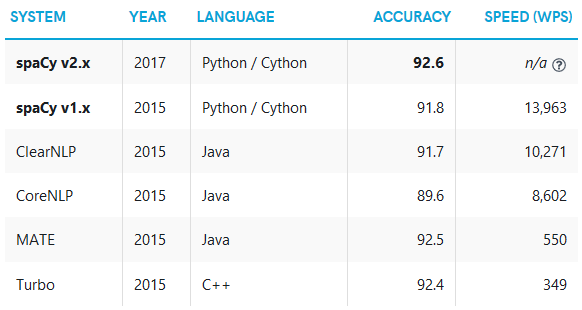
\includegraphics[width = 0.75\textwidth]{Imagenes/Bitmap/spacyeval.png}%
	\caption{Benchmarks of different syntactic parsers}%
	Image extracted from \url{https://spacy.io/usage/facts-figures#benchmarks}
	\label{fig:spacyeval}
\end{figure}

An evaluation published by \textit{Yahoo! Labs} and Emory University, as a part of a survey of current parsing technologies \citep{choi2015depends}, observed that ``spaCy is the fastest greedy parser'' and its accuracy is within 1\% of the best available (as we can see in Figure \ref{fig:spacyeval}). The few systems that are more accurate are 20 times slower or more.

\cite{choi2015depends} results and subsequent discussions helped spaCy develop a novel psychologically-motivated technique to improve spaCy's accuracy, which they published in joint work with Macquarie University \citep{honnibal2015improved}.

Besides, not only in general but in each particular task (tokenise, tag and parse), spaCy is the fastest if we compare it with other natural language processing libraries. This is shown in Figure \ref{fig:spacyspeed}, where we can observe both absolute timings (in ms) and relative performance (normalized to spaCy). Lower is better.

\begin{figure}[h]
	\centering%
	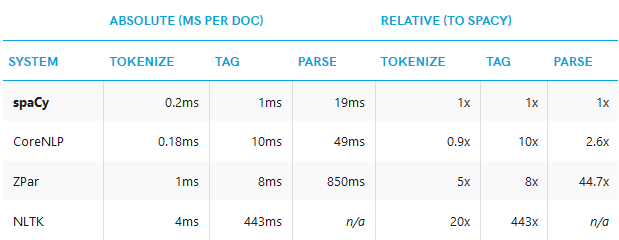
\includegraphics[width = 0.85\textwidth]{Imagenes/Bitmap/spacyspeed.png}%
	\caption{Per-document processing time of various NLP libraries}%
	Image extracted from \url{https://spacy.io/usage/facts-figures#benchmarks}
	\label{fig:spacyspeed}
\end{figure}

Finally, spaCy has three pretrained model pipelines for Spanish with a very high accuracy (see Figure \ref{fig:spacymodel}). These will help us to tokenise, tag and parse our messages in order to calculate the different style markers defined.

\begin{figure}[h]
	\centering%
	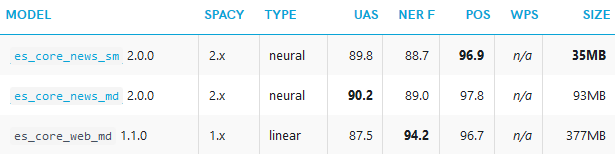
\includegraphics[width = 0.85\textwidth]{Imagenes/Bitmap/spacymodel.png}%
	\caption{Benchmark accuracies for the Spanish pretrained model pipelines}%
	Image extracted from \url{https://spacy.io/usage/facts-figures#benchmarks}
	\label{fig:spacymodel}
\end{figure}